\documentclass[10pt,a4paper]{article}
\usepackage{blindtext}
\usepackage{subcaption}
\usepackage{graphicx}
\usepackage{tikz}
\usepackage{amssymb}
\usepackage{caption}
\usepackage{amsmath}
\usepackage{circuitikz}
\usepackage{hyperref}
\usepackage{amssymb}
\usepackage{amsmath}
\usepackage{listings}
\lstset{
    inputencoding=utf8,
    extendedchars=true,
    literate={á}{{\'a}}1 {é}{{\'e}}1 {í}{{\'i}}1 {ó}{{\'o}}1 {ú}{{\'u}}1 {ñ}{{\~n}}1 {Á}{{\'A}}1 {É}{{\'E}}1 {Í}{{\'I}}1 {Ó}{{\'O}}1 {Ú}{{\'U}}1 {Ñ}{{\~N}}1
}
\input{AEDmacros}
\newcommand{\notimplies}{\;\not\!\!\!\implies}
\title{Análisis II}
\author{Tomás Agustín Hernández}
\date{}

\begin{document}
\maketitle

\begin{figure}[b]
    \centering
    \begin{tikzpicture}[remember picture,overlay]
        \node[anchor=south east, inner sep=0pt, xshift=-1cm, yshift=2cm] at (current page.south east) {
            \begin{minipage}[b]{0.5\textwidth}
                \includegraphics[width=\linewidth]{logo_uba.jpg}
                \label{fig:bottom}
            \end{minipage}
        };
    \end{tikzpicture}
\end{figure}
\newpage
\section*{Dilatación}
Sean $a, n \in \float $ decimos que estamos dilatando al número a sí y solo sí $ a \ = \ a \ * \ n$ con $n >= 1$
\section*{Contracción}
Sean $a, n \in \float $ decimos que estamos contrayendo al número a sí y solo sí $ a \ = \ a \ * \ n$ con $ 0 > n < 1$
\section*{Plano Real $\float^{2}$}
Se define como $\float^{2} = \float x \float = \{(a, b): a, b \in \float\}$
Aquí, los puntos se definen con dos coordenadas: x e y.
\section*{Plano Real $\float^{3}$}
También conocido como $espacio$. \\
Se define como $\float^{3} = \float x \float = \{(a, b, c): a, b, c \in \float\}$
\subsection*{Orientación de los ejes}
Se rigen por la regla de la mano derecha. Cuando vamos girando, hacia donde queda apuntando el dedo es el eje z.
\section*{Distancia entre dos puntos}
Sean dos puntos $P = (a_{1}, a_{2}) \ y \ Q = (b_{1}, b_{2})$, definimos la distancia entre dos puntos como "la distancia entre P y Q es la raíz cuadrada de la suma de los cuadrados de las diferencias de sus coordenadas." \\ 
\[dist(P,Q) = \sqrt[]{(b_{2} - a_{2})^{2} + (b_{1} - a_{1})^{2}}\]
Esta misma definición es generalizable para n coordenadas. \\
\textbf{Nota}: $dist(P, Q) = long(\bar{PQ})$

\section*{Circunferencias y Discos (Solo en $\float^{2}$)}
\subsection*{Circunferencia}
Sea un centro $C_{0} = (a_{0}, b_{0})$ y radio $r > 0$ definimos a una circunferencia como: 
\[\{(x, y) \in \float^{2}: \sqrt[]{(x - a_{0})^{2} + (y - b_{0})^{2} \textcolor{purple}{=} r}\}\] 

Si notamos que la circunferencia está definida usando la definición de distancia entre dos puntos, si desarrollamos la ecuación de la circunferencia nos queda algo así: 
\[(x-x_{1})^{2} + (y-x_{2})^{2} = r^{2}\]

\textbf{Importante}: La circunferencia \$' =  $\{(x, y) \in \float^{2}: \sqrt[]{x^{2} + y^{2} = 1}\}$ es conocida como Circunferencia Unidad.
\subsection*{Disco Abierto}
Cada vez que leamos la palabra $abierto$ quiere decir que no incluye los bordes, sino solo el contenido.
Definimos el Disco Abierto de centro $C_{0}$ y radio $r > 0$ como 
\[\{(x, y) \in \float^{2}: \sqrt[]{(x - a_{0})^{2} + (y - b_{0})^{2} < r}\}\]

\subsection*{Disco Cerrado}
Exactamente igual que el Disco Abierto pero con los bordes incluidos. \\ 
Definimos el Disco Abierto de centro $C_{0}$ y radio $r > 0$ como 
\[\{(x, y) \in \float^{2}: \sqrt[]{(x - a_{0})^{2} + (y - b_{0})^{2} \textcolor{purple}{\le} r}\}\]
\section*{Esferas y Bolas (Solo en $\float^{3}$)}
\subsection*{Esfera}
Sea un centro $ C_{0} = (a_{0}, b_{0}, c_{0})$ y radio $r > 0$ definimos una esfera como: 
\[\{(x, y, z) \in \float^{3}: \sqrt[]{(x_{0} - a_{0})^{2} + (y_{0} - b_{0})^{2} + (z_{0} - c_{0})^{2} \textcolor{purple}{=} r}\}\]
\subsection*{Definición formal de Esfera}
\[ Br(P) = \{X = (x_{1}, ..., x_{n}) \in \float^{n} : ||X-P|| = r\}\]
\begin{center}
    \begin{minipage}[b]{0.3\textwidth}
        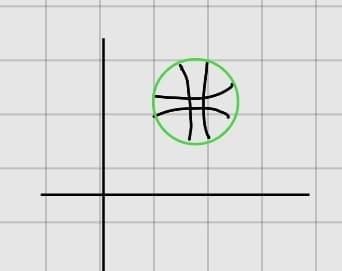
\includegraphics[width=\linewidth]{assets/esfera.jpg}
        \centering
        \label{fig:esfera}
    \end{minipage}
\end{center}
\subsection*{Bola Abierta}
Misma idea que Disco Abierto pero en $\float^{3}$
\[\{(x, y, z) \in \float^{3}: \sqrt[]{(x - a_{0})^{2} + (y - b_{0})^{2} + (z_{0} - c_{0})^{2} < r}\}\] 
\subsection*{Definición formal de Bola Abierta}
\[ Br(P) = \{X = (x_{1}, ..., x_{n}) \in \float^{n} : ||X-P|| < r\}\]
\begin{center}
    \begin{minipage}[b]{0.3\textwidth}
        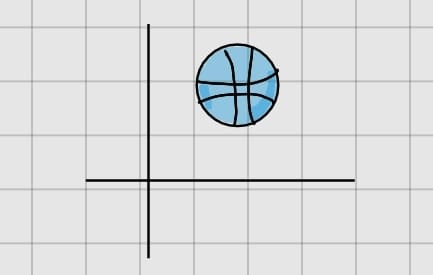
\includegraphics[width=\linewidth]{assets/bola_abierta.jpg}
        \centering
        \label{fig:bola_abierta}
    \end{minipage}
\end{center}
\subsection*{Bola Cerrada}
Misma idea que Disco Cerrado pero en $\float^{3}$
\[\{(x, y, z) \in \float^{3}: \sqrt[]{(x - a_{0})^{2} + (y - b_{0})^{2} + (z_{0} - c_{0})^{2} \ \textcolor{purple}{\le} \ r}\}\]
\textbf{Nota}: Véase $\hyperref[subsec:completar_cuadrados_esfera]{\underline{anexo}}$ para ver ejercicios de completar cuadrados y encontrar el centro y radio de una esfera.
\subsection*{Definición formal de Bola Cerrada}
\[ Br(P) = \{X = (x_{1}, ..., x_{n}) \in \float^{n} : ||X-P|| \le r\}\]
\begin{center}
    \begin{minipage}[b]{0.3\textwidth}
        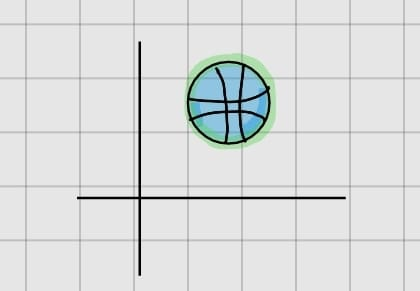
\includegraphics[width=\linewidth]{assets/bola_cerrada.jpg}
        \centering
        \label{fig:bola_cerrada}
    \end{minipage}
\end{center}
\section*{Aclaración sobre enunciados}
Importante siempre prestar atención a la dimensión donde trabajamos. \\
Es decir $x^{2} + y^{2} = 4$ puede representar dos cosas diferentes si estamos en $\float^{2}$ o en $\float^{3}$
\section*{Vectores}
Los vectores tienen dirección, sentido y longitud. \\
Sean dos puntos $P, Q \in \float^{n}$, definimos un vector $V \in \float^{n}$ como $ \bar{PQ} = Q - P$.
\subsection*{Vectores Equivalentes}
Dos vectores son equivalentes si tienen misma dirección, sentido y longitud. 
\subsection*{Vectores Iguales}
Dos vectores son iguales si son equivalentes y además parten del mismo punto.
\subsection*{Suma de Vectores}
Sean $ u, v $ vectores $\in \float^{n}$. La suma de ambos se realiza coordenada a coordenada.
$ u + v = (u_{1} + v_{1}, u_{2} + v_{2}, ..., u_{n} + v_{n})$
\subsection*{Producto por Escalar}
Sea $t \in \float$ y u un vector.
$ t * u = (tu_{1}, tu_{2}, ..., tu_{3})$
\subsection*{Regla del Paralelo}
Se utiliza para ver como queda la traslación del vector $u+v$ luego de sumar ambos vectores.
\subsection*{Propiedades de los vectores}
\begin{itemize}
    \item La suma es conmutativa: u + v = v + u
    \item Sea un valor $ t \in \float $, definimos la distributiva con vectores como t(u+v) = tu + tv
\end{itemize}
\subsection*{Norma de un Vector}
Definimos la norma de un vector como $ || V || = \sqrt[]{(v_{1})^{2} + (v_{2})^2 + ... + (v_{n})^2}$ 
\subsection*{Relación entre distancia entre dos puntos y la norma}
Es fácil notar que $ ||B-A|| = ||A-B||. $ 
Definimos la \textbf{equivalencia} de las siguientes fórmulas: 
\[ dist(A, B) = ||B-A|| \equiv ||A-B|| \]
\subsection*{Propiedades de la norma}
\begin{itemize}
    \item $||V||  \ge  0$
    \item $|V| = \sqrt[]{V^{2}}$
    \item $||V|| = dist(V, 0)$
    \item $\alpha \in \float, ||\alpha * V|| = ||\alpha|| * ||V||$: en criollo quiere decir que si multiplico un escalar dentro de la norma, es lo mismo que sacarlo hacia afuera y hacerlo por separado. 
    \item $||V+W|| \le ||V|| + ||W||$: desigualdad Triangular (DT)
    \item $||V-W|| \le ||V|| + ||-W||$: esto tiene sentido pues $||-w||$ es positivo. Entonces queda $||V-W|| \le ||V|| + ||W||$
    \begin{itemize}
        \item Importante: Esto se utiliza mucho para acotar. $ ||V+W||$ y $||V-W||$ se acotan por $ ||V|| + ||-W|$
    \end{itemize}
\end{itemize}
\textbf{Importante}: Si aplico la NORMA a un número, es como aplicar el módulo.
\section*{Producto Interno (Producto Escalar / Producto Punto)}
Sean $u, v \in \float^{n}$. Definimos el producto interno, como la multiplicación \textbf{coordenada a coordenada} de los vectores. \textbf{Siempre devuelve un número.} \\
Hay dos formas de notarlo
\[<u,v> = u * v\]
\subsection*{Vectores Perpendiculares}
Sean $u, v \in \float^{n}$. Si el producto escalar entre dos vectores es 0, entonces los vectores son perpendiculares.
\subsection*{Propiedades del Producto Interno}
\begin{itemize}
    \item $u * u = ||u||^{2}$
    \item Conmutatividad: $u * v = v * u$
    \item Distributividad: Sean $u, v, w \in \float^{n}$, entonces $(u+v) * w = uw + vw$ 
    \item $ t \in \float, (t * u) * v = t * (u * v) = u * (t * v)$
\end{itemize}
\textbf{Importante}: No se pueden multiplicar 3 vectores con el producto interno, porque el producto interno devuelve un NÚMERO. Si multiplico 3 vectores, sería multiplicar primero dos (devuelve un número) y según si es $ > 1 $ o no, estaríamos dilatando/contrayendo otro vector. 
\subsection*{Propiedad importante de la norma y el Producto Interno}
Sean $v, w \in \float^{n}$
\[ v * w = ||v|| * ||w| * cos(\theta)\] con $ 0 \le \theta \le \pi $
\subsection*{Teorema de Cauchy-Schwartz}
$\forall u, v \in \float^{n}$ vale $ |u * v| \le ||u|| * ||v||$
\textbf{Importante}: Si $|u * v| = ||u|| * ||v||$ entonces $ v // u$ (v es paralelo a u)
\section*{Proyecciones}
Sean $v, w \in \float^{n}$. Queremos calcular la proyección de w en la dirección de v. 
\[P_{v}(w) = w * \frac{v}{||w||} * \frac{v}{||v||} = w * v * \frac{v}{||v||^{2}} = \frac{w * v}{v * v} = \frac{w * v}{v^{2}} * v\]
\section*{Producto Vectorial / Cruz (Solo en $\float^{3}$)}
Sean $v, w \in \float^{3}$. Se utiliza para calcular un \textbf{vector perpendicular} a los dos que se nos envían.
\[
\begin{pmatrix}
\hat{i} & \hat{j} & \hat{k} \\
a & b & c\\
d & e & f
\end{pmatrix}
\]
Entonces, el cálculo que hay que hacer es: ((b * f) - (c * e), \textcolor{red}{-} ((a * f) - (c * d)), ((a * e) - (b * d)))
\textbf{Importante}: Si este cálculo da 0, entonces los vectores son paralelos.
\subsection*{Propiedades del Producto Vectorial}
\begin{itemize}
    \item (V x W) es perpendicular a V y W.
    \begin{itemize}
        \item Esto es re útil para cuando encontramos una normal para el plano y queremos ver si efectivamente es perpendicular a ambos vectores.
    \end{itemize}
    \item (W x V) = - (V x W): Es decir, no son iguales si los invertimos, si lo invierto le cambio el signo. 
\end{itemize}
\section*{Planos en $\float^{3}$}
Dado un \textbf{vector normal N} y un \textbf{punto de paso P} construimos la ecuación del plano $\pi$ que es perpendicular al \textbf{vector normal} y contiene al punto P (es decir, P verifica la ecuación del plano).
Véase \textbf{\hyperref[subsec:ejercicios_planos]{\underline{anexo}}} para ejercicios de Planos.
\subsection*{Hallar vector normal N de un Plano}
El vector normal N de un Plano lo podemos hallar comúmnente de las siguientres maneras 
\begin{itemize}
    \item Si tenemos 3 puntos, ABC podemos hacer la diferencia y generar 2 vectores directores. Es decir, AB y BC o AB y AC. Luego aplicamos el producto cruz y ya tenemos la normal al plano. Por último podemos tomar cualquier punto.
    \begin{itemize}
        \item Como tenemos la NORMAL tenemos (a, b, c) nos falta d. Para generar d podemos evaluar ax + by + cz con cualquier punto de paso. El número que da como resultado es d.
    \end{itemize}
\end{itemize}
\subsection*{Ecuación Paramétrica del Plano}
$ \pi: \lambda(x_{1}, x_{2}, x_{3}) + \gamma(y_{1}, y_{2}, y_{3}) + (p_{1}, p_{2}, p_{3})$
\subsection*{Ecuación Implícita del Plano}
$ \pi: ax + by + cz = d$
\subsection*{Saber si un punto está en un plano}
Debe verificar la ecuación implícita.
\section*{Rectas Paramétricas}
En $\float^{2} = L:(x,y) = \alpha (v_{1}, v_{2}) + (P_{1}, P_{2}), \alpha \in \float$ \\
En $\float^{3} = L:(x,y,z) = \alpha (v_{1}, v_{2}, v_{3}) + (P_{1}, P_{2}, P_{3}), \alpha \in \float$
Véase \hyperref[subsec:ejercicios_rectas_planos]{\underline{anexo}} para ver ejercicios con rectas y planos.
\subsection*{Rectas Paralelas}
Dos rectas son paralelas sí sus vectores son uno múltiplo del otro.
\subsection*{Rectas Perpendiculares}
Dos rectas son perpendiculares si el producto escalar entre ambos vectores directores da 0.
\subsection*{Rectas Alabeadas}
Dos rectas son alabeadas si no existe intersección entre ellas, y además son paralelas.
\subsection*{Intersección entre dos rectas}
Sean $L_{1}, L_{2}$ dos rectas.
La intersección entre dos rectas se da en un punto específico. Por lo tanto, se espera que la intersección sea un número y además, este número pertenece a $L_{1}$ Y $L_{2}$
\subsection*{Casos de Rectas y Planos}
\begin{itemize}
    \item Si tengo plano + 2 rectas: Si se cruzan o son paralelas, entonces existe un único plano.
    \item Si tengo plano + 1 recta: Existen infinitos planos que la contenga.
\end{itemize}
\section*{Curvas}
Son un conjunto de puntos por los que pasó una partícula dada a lo largo del tiempo.
La trayectoria, el movimiento que hace en cada tiempo t la partícula va dejando una marca y forma una curva. \\
Las funciones son de la forma 
\[
f(t) =
\begin{cases} 
x = x(t) \\
y = y(t)
\end{cases}
\]
\textbf{Nota}: Una recta es un tipo de curva. Donde un punto puede hacer una trayectoria de manera ascendente o descendente.
\subsection*{Paramétrización de la Curva}
Existen infinitas parametrizaciones para una misma curva. Esto quiere decir, que una misma partícula puede realizar una trayectoria de mil maneras diferentes. \\
Denotamos la parametrización de una curva como: $C = \{(x(t), y(t)) \ / \ t \in \float \}$ y decimos que es paramétrica porque espera un parámetro.
\subsection*{¿Qué no nos dice la ecuación implícita de una curva?}
Las ecuaciones en x y y describe \textbf{donde} ha estado la partícula pero no nos dice \textbf{cuándo} ha estado la partícula en un punto en particular. 
\subsection*{¿Qué nos dice la ecuación paramétrica de una curva?}
La ventaja es que nos dicen \textbf{cuándo (t)} estuvo la partícula en un punto (x, y) y la dirección en su trayectoria.
\subsection*{Ejemplo de Curvas}
Recordemos que básicamente una curva se arma gracias a la trayectoria de una partícula que hace cierto movimiento a lo largo del tiempo. \\
Este tiempo se llama t, y podemos ir viendo el movimiento de la partícula gracias a la ecuación paramétrica. A medida que t aumenta, esa es la dirección que toma la partícula. \\
\[
f(t) =
\begin{cases} 
x = t^{2} - 2t \\
y = t - 1
\end{cases}
\]
Si nos ponemos a darle valores a t, vamos a ir obteniendo valores de x e y, que básicamente los podemos graficar en un plano.
\[\begin{minipage}[b]{0.7\textwidth}
    \includegraphics[width=\linewidth]{assets/curva.png}
\end{minipage}\]
Parece entonces en este ejemplo, que la partícula hizo la trayectoria de una parábola. Busquemos entonces la ecuación implícita para ver qué curva representan las ecuaciones paramétricas.
\[
f(t) =
\begin{cases} 
x = t^{2} - 2t \\
y = t - 1 \equiv y+1 = t
\end{cases}
\]
Entonces, $ x = (y+1)^{2} - 2(y+1) \equiv x = y^{2} -4y +3$ \\
Efectivamente podemos notar que la partícula, gracias a esas ecuaciones parámetricas y dando el tiempo t fuimos formando la curva paramétrica (parábola) $ x = y^{2} -4y +3$. \\
Entonces ¿cuál es la diferencia entre tener la ecuación paramétrica con un parámetro t o tener la que depende de x e y? La diferencia es que con la parámetrica podemos saber en qué lugar estaba la partícula en un tiempo t. \\
\subsection*{Restringiendo los posibles valores t de la Curva}
Se utilizan intervalos. Es decir, nosotros podemos decir qué trayectoria recorre la partícula, desde qué t hasta qué t. \\
Esto se define como $ x = f(t) \ y \ y = g(t) \ a \le t \le b$ donde el \textbf{punto inicial} es (f(a), g(a)) y el \textbf{punto final} es (f(b), g(b)). \\
Ejemplo: $ x = (t^{2} - 2t) \ y = (t+1) \ 0 \le t \le 4$
\[\begin{minipage}[b]{0.5\textwidth}
    \includegraphics[width=\linewidth]{assets/curva_delimitada.png}
\end{minipage}\]
\subsection*{Circunferencias Paramétricas}
Se suelen representar con coseno y seno.
\[x = cos(t), y = sen(t), 0\le t \le 2\pi\]
Si damos unos valores t y dibujamos en el plano, veremos que está realizando una circunferencia de radio 1.
\[\begin{minipage}[b]{0.5\textwidth}
    \includegraphics[width=\linewidth]{assets/cost_sent.png}
\end{minipage}\]
Observamos que $x^{2} + y^{2} = cos^{2}\ t + sen^{2}\ t = 1$. En este caso la circunferencia se va completando gracias a la trayectoria del punto que va en sentido antihorario. \\
\[x = sen(2t), y = cos(2t), 0\le t \le 2\pi\]
Este es parecido al anterior, la diferencia es que ahora vamos al \textbf{doble de velocidad}. Antes con cos(t) y sen(t) ibamos de 0 a 2pi \textbf{una vez}. Acá, al estar multiplicado el t por 2, lo que va a hacer es que vamos a recorrer en 2pi \textbf{dos veces} la circunferencia (cada $\pi$ recorrimos la circunferencia entera). Pero ojo, esta es sen(2t) y cos(2t) entonces, está invertido el recorrido. Acá se hace en sentido horario.
\[\begin{minipage}[b]{0.7\textwidth}
    \includegraphics[width=\linewidth]{assets/sen2t_cos2t.png}
\end{minipage}\]
Nótese que llegamos a 3.14 y ya recorrió toda la circunferencia gracias al 2t (antes recorría la mitad). Sin embargo, el deslizador indica que le falta todavía una vuelta para dar. \\
\textbf{Conclusión}: Podemos ver que dos parametrizaciones diferentes, representan la misma curva (circunferencia), pero recorrida a diferente velocidad.
\subsection*{Deslizadores en GeoGebra}
Nos permiten simular como una partícula se mueve realizando la curva. \\
\[\begin{minipage}[b]{0.9\textwidth}
    \includegraphics[width=\linewidth]{assets/geogebra.png}
\end{minipage}\]
Por si requiere orientación, observe este \href{https://www.youtube.com/watch?v=Sb1W73Vb_98&list=PLvwXmp0qN7l2Fg-D4eWt57Fri_fYN-Sw5&index=2&t=671s}{vídeo}.
\[\begin{minipage}[b]{0.9\textwidth}
    \includegraphics[width=\linewidth]{assets/resultado_geogebra_curva.png}
\end{minipage}\]
\section*{Coordenadas Cartesianas y Polares}
\subsection*{Coordenada Cartesiana}
Permite representar un punto en el plano mediante un par ordenado de números llamados coordenadas. \\
Ej.: $P = (1, 2)$ está dado de forma cartesiana.
\subsection*{Coordenada Polar}
Permite representar un punto P mediante el par ordenado $(r, \theta)$ y r, $\theta$ se llaman coordenadas polares de P. \\
\textbf{Recordatorio}: r: largo, $\theta$: ángulo desde el (0, 0)
\[\begin{minipage}[b]{0.3\textwidth}
    \includegraphics[width=\linewidth]{assets/coordenadas_polares.png}
\end{minipage}\]
\textbf{Nota}: Si $r>0$ el punto $(r, \theta)$ está en el mismo cuadrante que $\theta$. Si $r<0$ está en el cuadrante opuesto del polo $(-r, \theta) \equiv (r, \theta + \pi)$
\[\begin{minipage}[b]{0.3\textwidth}
    \includegraphics[width=\linewidth]{assets/coordenadas_polares_2.png}
\end{minipage}\]
\subsection*{Coordenadas Polares a Cartesianas}
La fórmula se deduce a partir de lo siguiente $ cos \ (\theta) \ = \ \frac{x}{r} \ , \ sen(\theta) = \frac{y}{r}$
\[\begin{minipage}[b]{0.3\textwidth}
    \includegraphics[width=\linewidth]{assets/coordenadas_polares_a_cartesiana.png}
\end{minipage}\]
Masajeando un poco, nos queda
\[x = r * cos(\theta), \ y = r * sen(\theta)\]
\subsection*{Coordenadas Cartesianas a Polares}
Podemos calcularlo a partir del pasaje o la figura anterior. Por lo tanto nos quedaría 
\[r^{2} = x^{2} + y^{2},\ tan(\theta) = \frac{y}{x} \]
Véase \hyperref[subsec:pasaje_coord_polares_cartesianas]{anexo} para ejercicios acerca de los pasajes en este tema. 
\section*{Curvas Polares}
La gráfica de una ecuación polar $r = f(\theta)$ o de manera más general $F(r, \theta) = 0$ consiste de todos los puntos P que tienen al menos una representación polar $(r, \theta)$. \\
\textbf{Ej.}: $ r = 2 $ representa a $F(2, \theta)$ y esto sería básicamente una circunferencia con centro 0 y de radio 2. ¿Por qué una circunferencia? Porque $\theta$ es un ángulo, y los ángulos van desde $0\le \theta \le 2\pi$
\[\begin{minipage}[b]{0.9\textwidth}
    \includegraphics[width=\linewidth]{assets/curvas_polares_graficos.png}
\end{minipage}\]
En la imagen anterior podemos ver varias curvas polares que representan circunferencias con centro 0. \\
\newpage
\textbf{Ej.}: $ \theta = 1$ representa a una curva que posee siempre el ángulo $\theta = 1 \ (medido \ en \ radianes)$ sin ninguna restricción acerca de p. 
\[\begin{minipage}[b]{0.6\textwidth}
    \includegraphics[width=\linewidth]{assets/curva_polar_solo_angulo.png}
\end{minipage}\]
\subsection*{Pasaje de Curva dada en forma Polar a Curva dada en Ecuación Cartesiana}
\[\begin{minipage}[b]{0.7\textwidth}
    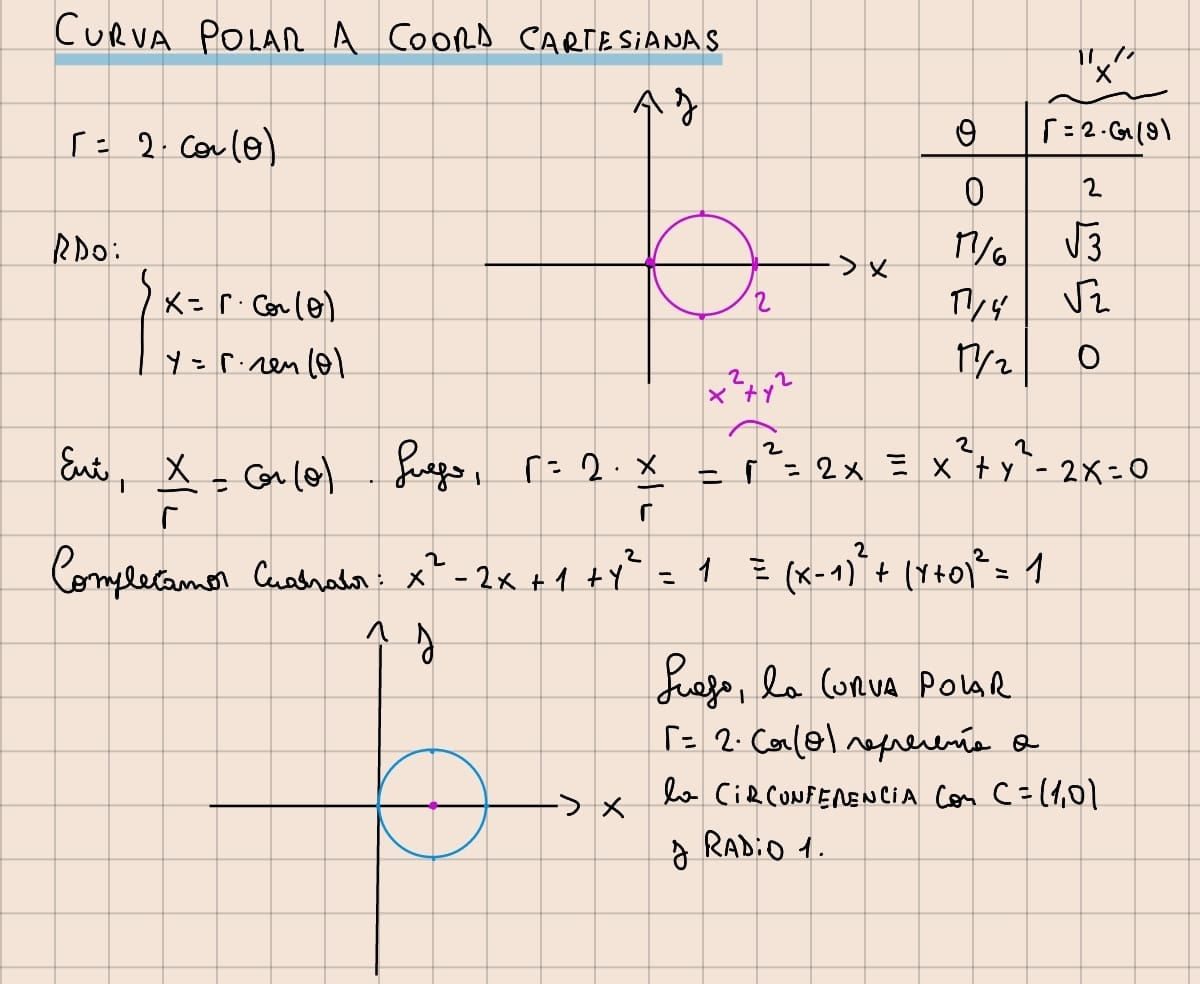
\includegraphics[width=\linewidth]{assets/curva_polar_a_coord_cartesianas.jpg}
\end{minipage}\]
\textbf{Importante}: Véase que despejamos $x = r * cos(\theta)$ para ver qué vale $cos(\theta)$ porque nuestro ejercicio tenia un $2 * cos(\theta)$. Nos queda más fácil para aplicar $r^{2} \equiv x^{2} + y^{2}$
\subsection*{Cardioide}
\[\begin{minipage}[b]{0.5\textwidth}
    \includegraphics[width=\linewidth]{assets/cardioide.png}
\end{minipage}\]
\subsection*{Rosa de 4 Pétalos}
\[\begin{minipage}[b]{0.6\textwidth}
    \includegraphics[width=\linewidth]{assets/rosa_4_petalos.png}
\end{minipage}\]
\textbf{Preguntar}: ¿Por qué $ r = 2 * cos(\theta)$ es fácil pasarlo a ecuación cartesiana y no pasa lo mismo con $ r = 1 + sen(\theta) $ o $ r = cos(2 \theta)$?
\section*{Cónicas}
Se llaman cónicas porque resultan de cortar un cono con un plano. 
\subsection*{Parábolas}
Una parábola es el conjunto de puntos en el plano que estan a igual distancia de un punto fijo F (llamado \textbf{foco}) y una recta fija (llamada \textbf{directriz}). \\
El punto entre el foco y la directriz se llama \textbf{vértice}. \\
La recta perpendicular a la directriz que pasa por el foco se llama \textbf{eje} de la parábola.
\[\begin{minipage}[b]{0.4\textwidth}
    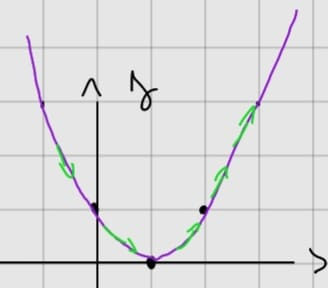
\includegraphics[width=\linewidth]{assets/parabola.png}
\end{minipage}\]
\subsection*{Relación entre el Foco y la Directriz}
Si el foco está en el punto $(0, p)$ entonces la directriz tiene la ecuación $y = -p$. 
Esto quiere decir que la \textbf{distancia del foco al vértice} es la \textbf{misma} que la \textbf{distancia de la directriz al vértice.}
\subsection*{Distancia de un punto $P(x, y)$ de la parábola al Foco y Directriz}
\textbf{P a Foco}: $|PF| = \sqrt[]{x^{2} + (y-p)^{2}}$ \\
\textbf{P a Directriz}: $ |y+p| = \sqrt[]{x^{2} + (y-p)^{2}} $ \\
La ecuación equivalente que se consigue desarrollando $ |y+p| = \sqrt[]{x^{2} + (y-p)^{2}} $ es $x^{2} = 4py \equiv \frac{1}{4p} x^{2} = y \equiv ax^{2} = y  $
\subsection*{Parametrizando una Función}
Consideremos $ax^{2} = y$, la manera de parametrizarla es de la siguiente forma 
\[
f(t) =
\begin{cases} 
x = t \\
y = at^{2}
\end{cases}
\]
\subsection*{Efecto del Foco y la Directriz con la Parábola}
Más cerca esté de origen el punto P, entonces más chica será la distancia entre el foco y la directriz y la parábola será menos ancha. 
\[\begin{minipage}[b]{0.6\textwidth}
    \includegraphics[width=\linewidth]{assets/parabola_1.png}
\end{minipage}\]
\[\begin{minipage}[b]{0.6\textwidth}
    \includegraphics[width=\linewidth]{assets/parabola_2.png}
\end{minipage}\]
\subsection*{¿Hacia donde abre la parábola?}
\begin{itemize}
    \item $x^{2} = 4py$ (directriz en y, foco (0, p))
    \begin{itemize}
        \item $p > 0$: Hacia arriba
        \item $p < 0$: Hacia abajo
    \end{itemize}
    \item $y^{2} = 4px$ (directriz en x, foco (p, 0))
    \begin{itemize}
        \item $p>0$: Hacia la derecha
        \item $p<0$: Hacia la izquierda
    \end{itemize}
\end{itemize}
\textbf{Recordatorio}: La directriz y el foco están en el eje contrario al que tiene el cuadrado.
\subsection*{Elipses}
Una elipse es el conjunto de planos en un plano cuya suma de sus distancias a dos puntos $F_{1}$ y $F_{2}$ es una constante. Estos dos puntos fijos se llaman \textbf{focos}. 
\subsection*{Cálculo de los focos}
La fórmula es: $c^{2} = a^{2} - b^{2}$
\subsection*{Formas de armar una Elipse}
Existe un concepto que es eje mayor y eje menor. Encontrando el eje mayor ya sabemos donde están posicionados los focos y los vértices. \\
$\frac{x^{2}}{a^{2}} + \frac{y^{2}}{b^{2}} = 1 \ con \ a \ge b > 0$: tiene focos $(\pm c, 0)$ donde $c^{2} = a^{2} - b^{2}$ y vértices $(\pm a, 0)$ \\
$\frac{x^{2}}{b^{2}} + \frac{y^{2}}{a^{2}} = 1 \ con \ a \ge b > 0$: tiene focos $(0,  \pm c)$ donde $c^{2} = a^{2} - b^{2}$ y vértices $(0, \pm a)$ \\
\textbf{En criollo}: La letra que tiene un denominador más grande, es el que tiene los focos y el vértice (eje mayor). El eje mayor sería hacia donde es más grande. El número más grande siempre es \textbf{a}. \\
\textbf{Tips}: Siempre recordar que si me dan un foco ya puedo determinar el eje mayor; mismo con si me dan un vértice. Recordar también que el vértice depende de \textbf{a} esto quiere decir es que si me dan el vértice me dieron el eje mayor. \\
En la teoría no hay más que eso, véase \hyperref[subsec:elipses_ejercicios]{anexo} para ver ejercicios de elipses. \\
\subsection*{Hipérbolas}
Una Hipérbola es el conjunto de todos los puntos en un plano cuya diferencia de sus distancias a dos puntos fijos $F_{1}$ y $F_{2}$ (los focos) es una constante. \\
\subsection*{Cálculo de los focos}
La fórmula es: $c^{2} = a^{2} + b^{2}$
\subsection*{Formas de armar una Hipérbola}
Existe un concepto que es eje mayor y eje menor. Encontrando el eje mayor ya sabemos donde están posicionados los focos y los vértices. \\
$\frac{x^{2}}{a^{2}} - \frac{y^{2}}{b^{2}} = 1 \ con \ a \ge b > 0$: tiene focos $(\pm c, 0)$ donde $c^{2} = a^{2} + b^{2}$, vértices $(\pm a, 0)$ y asíntotas $y = \pm \frac{b}{a}x$ \\
$\frac{x^{2}}{b^{2}} - \frac{y^{2}}{a^{2}} = 1 \ con \ a \ge b > 0$: tiene focos $(0,  \pm c)$ donde $c^{2} = a^{2} + b^{2}$, vértices $(0, \pm a)$ y asíntotas $y = \pm \frac{a}{b}x$ \\
En la teoría no hay más que eso, véase \hyperref[subsec:hiperbolas_ejercicios]{anexo} para ver ejercicios de elipses. \\
\section*{Cónicas Desplazadas}
Son exactamente las mismas maneras, solo que acá en vez de x e y es (x-k) y (y-k).
Entonces, ej hipérbola con eje mayor x
\begin{itemize}
    \item $vertices = (centroX \pm a, centroY)$
    \item $focos = (centroX \pm c, centroY)$
    \item $hiperbolas = -\frac{b}{a}(x - centroX) \ y \ \frac{b}{a}(x - centroX) $
\end{itemize}

\section*{Anexo}
\subsection*{Esferas}
\label{subsec:completar_cuadrados_esfera}
Complete y lleve a una fórmula conocida: $x^{2} + y^{2} + z^{2} + 8x - 6y + 16$ 
\begin{itemize}
    \item Reordeno: $x^{2} + 8x + y^{2} - 6y +z^{2} = -16$ 
    \item Completo cuadrados, los valores que tienen la variable (sin exponente), hago $(num/2)^{2}$.
    \begin{itemize}
        \item $(x^{2} + 8x + 16) + (y^{2} - 6y + 9) + z^{2} - 16 - 9 = -16$
        \item Nótese que como nos inventamos términos para completar cuadrados, tenemos que restarlos.
    \end{itemize}
    \item Reordeno: $(x^{2} + 8x + 16) + (y^{2} - 6y + 9) + z^{2} = -16 + 16 + 9$
    \item Para agrupar un cuadrado, el numero que no tiene variable, tengo que aplicarle la raíz cuadrada. Luego, el símbolo que los separa es el signo del coeficiente que tiene variable grado uno.
    \begin{itemize}
        \item $(x+4)^{2} + (y-3)^{2} + z^{2} = 9$
    \end{itemize}
    \item Por último, como el radio está elevado al cuadrado lo reducimos $(x+4)^{2} + (y-3)^{2} + z^{2} = 3$
    \item El resultado entonces, es una Esfera en $\float^{3}$ con centro = (-4, 3, 0) y radio = 3
    \item Si se quisiera verificar si está bien, podemos desarrollar todos los cuadrados y deberíamos volver a la expresión original.
\end{itemize}
\subsection*{Completar Cuadrados}
Adjunto otro ejercicio que es de cónicas, pero acá tuve que completar cuadrados de una manera ligeramente diferente. \\
La forma de encararlo fue dejar el valor que esta solo del lado positivo. \\
Luego, como tuve que sacar factor común de las letras, al tener que completar los cuadrados lo que le tengo que restar es el factor común * el valor que agregué. Eso es lo que termino restando. 
\[\begin{minipage}[b]{0.9\textwidth}
    \includegraphics[width=\linewidth]{assets/completar_cuadrados.png}
\end{minipage}\]
\subsection*{Planos}
\label{subsec:ejercicios_planos}
\textbf{1}. Hallar la ecuación implícita del plano $\pi$ cuya normal sea $N=(-3, 0, 4)$ y que pasa por el punto $P=(2, 1, 1)$ \\
Recordemos como podemos armar un plano. Para poder armar un plano necesitamos un vector normal y un punto de paso. \\
Por lo tanto, este ejercicio es bastante simple, podemos simplemente aplicar la fórmula de $\pi:ax+by+cz = d$ \\
Entonces, nos quedaría algo así: $ \pi:-3x + 0y + 4z = d$ \\
Ahora ¿como calculo d?, podemos calcular d evalúando el punto $P$ en el plano. \\
Por lo tanto $d=-3(2) + 4(1) \equiv d = -2$ \\
Entonces, el plano $\pi:-3x+4z=-2$ \\

\textbf{2}. Dados los puntos $A=(1, 2, 3), B=(1,0,1) \ y \ C=(4, -1, 2)$ encuentre el plano. \\
Recordemos como podemos armar un plano. Para poder armar un plano necesitamos un vector normal y un punto de paso. \\
¿Tenemos la normal? No. ¿Como podemos calcularla? La manera de calcular un vector normal sería hacer el producto cruz entre dos vectores directores. \\
Por lo tanto, calculemos nuestros dos vectores directores $ \bar{AB} = (0, -2, -2)$ luego $\bar{BC} = (3, -1, 1)$ \\
\textbf{Nota}: Sería lo mismo calcular AB y BC que AB Y AC.
Ahora lo que podemos hacer es una vez que tenemos las dos direcciones podemos buscar con el producto cruz, un vector perpendicular que hará de nuestra normal. \\
PD: Recordemos que $A x B = - (B x A)$. Por lo tanto da igual que orden pongamos los vectores.
\[
\begin{pmatrix}
\hat{i} & \hat{j} & \hat{k} \\
0 & -2 & -2\\
3 & -1 & 1
\end{pmatrix}
\]
Nuestro vector normal N termina siendo N = $(-4, 6, 6)$ \\
¿Ahora qué nos falta? Un punto. Entonces podemos elegir cualquiera de los puntos A, B, C (xq las rectas estarían contenidas en el plano) \\
Si quisieramos verificar si efectivamente la normal nos dió bien, podemos calcular el producto escalar de $N * AB$ y $N * BC$ y ambos deberían dar 0. \\
Entonces, ahora por último hacemos lo mismo que en ejercicio anterior. $\pi:-4x+6y+6z=d \implies d=-4(1)+6(0)+6(1) \implies d = 2$ \\
Finalizamos, juntando la ecuación $\pi:-4x+6y+6z=2 \equiv \pi:-2x+3y+3z=1$ 
\subsection*{Rectas $\&$ Rectas y Planos}
\label{subsec:ejercicios_rectas_planos}
\textbf{1}. Dadas la recta $L:t(1, 1, 1) + (3, 0, 4)$ y el plano $\pi:2x-y+5z=10$ halle $L \cap \pi$. \\
Recordemos qué significa que una recta pueda intersecarse con un plano: que una recta pueda intersecarse con un plano o al revés significa que existe al menos un punto que tienen en común. \\
Con esto quiero decir que el punto que encontremos debe verificar tanto el plano como la recta. \\
Como tenemos que encontrar UN PUNTO necesitamos encontrar la fórmula generadora de puntos de la recta o el plano. \\
En este caso, como tenemos la recta en parámetrica y el plano en implícita nos conviene más fácil pasar la parámetrica y ver qué pinta tienen los puntos. \\
Entonces, si pasamos L a parámetrica nos queda: $(t+3, t, t+4)$ entonces $x=(t+3), y=t, z=t+4$ \\
Ahora, coloquemos lo que acabamos de encontrar en el plano, esto nos dará la variable $t$ para la recta. Como este t nos lo da después de meterlo el punto de la recta en el plano, cuando reemplacemos en el punto genérico con el t que encontramos, entonces ese punto será el de la intersección del plano y la recta.  \\
$\pi:2(t+3)-(t)+5(t+4)=10 \equiv \pi:2t+6-t+5t+20=20 \equiv \pi:t=\frac{-8}{3}$ \\
Ahora, este t lo colocamos en la fórmula genérica de los puntos de la recta: $((\frac{-8}{3}+3), \frac{-8}{3}, \frac{-8}{3}+4)$. \\
Entonces, la intersección es el punto $P=(\frac{1}{3}, \frac{-8}{3}, \frac{4}{3})$ \\
Por lo tanto, verifiquemos ahora, si este punto verifica el plano. \\
$\pi:2(\frac{1}{3}) - (\frac{-8}{3}) + 5(\frac{4}{3}) = 10 \equiv 10 = 10$

Luego, como el punto lo arrojó la recta, y verifica el plano, entonces la intersección $ L \cap \pi = (\frac{1}{3}, \frac{-8}{3}, \frac{4}{3})$ \\

\textbf{2}. Dar la ecuación implícita del plano $\pi$ que contiene a la recta. \\
$L:\alpha(2, 1, 3) + (2, 1, 0)$ y al punto $P=(0, 1, -1)$
Recordemos que si un plano contiene a una recta, todos los puntos de la recta están en el plano. \\
(preguntar qué pasaba si el punto estaba en la recta, qué cambiaba el ejercicio, en este caso no está)
Lo primero que tenemos que ver es si el punto $P \in L$. Si el punto está en la recta, entonces hay infinitos planos. Si el punto NO está en la recta, entonces hay un único plano. \\
Como necesito sí o sí dos vectores directores para mi plano, puedo hacer un vector director de la resta de $QP=(0, 1, -1) - (2, 1, 0) = (-2, 0, -1)$ \\
Entonces ahora hago el producto cruz entre $(2, 1, 3)$ y $(-2, 0, 1)$
\[
\begin{pmatrix}
\hat{i} & \hat{j} & \hat{k} \\
-2 & 0 & -1\\
2 & 1 & 3
\end{pmatrix}
\]
Nuestro vector normal N termina siendo N = $(1, 4, -2)$  \\
Entonces ahora, finalizamos el ejercicio evaluando en la normal el punto P $\pi:x+4y-2z=d$ \\
$d = (0) + 4(1) - 2(-1) \equiv d = 6$ \\
Entonces finalizamos con $\pi:x+4y-2z=6$ \\

\textbf{3}. Dadas las rectas $L_{1}:\alpha(-1, 0, 1) + (4, 3, 2)$ y $L_{2}:\gamma(2, 0, -2) + (0, 0, 1)$. Halle la ecuación implícita del plano $\pi$ que las contiene. \\
Lo primero que vemos es que tenemos dos rectas. Necesitamos de alguna manera un vector normal para el plano. \\
Primero vemos qué relación hay entre las rectas, podemos ver que son paralelas porque si hacemos $(-1, 0, 1) * -2$ nos da $(2, 0, -2)$. \\
Como son paralelas, necesitamos de alguna manera, llegar desde una recta a la otra, para luego, cuando tenemos un punto que llega y combina las rectas, ahí si podemos calcular con el producto cruz el vector normal. \\
\begin{center}
    \begin{minipage}[b]{0.6\textwidth}
        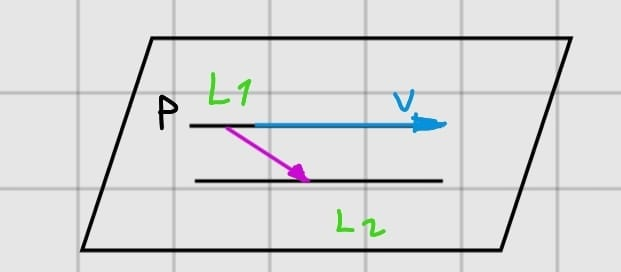
\includegraphics[width=\linewidth]{assets/rectas_paralelas_plano.jpg}
        \centering
        \label{fig:rectas_paralelas_plano}
    \end{minipage}
\end{center}
Entonces, restemos los dos puntos $\bar{PQ}=Q-P=(0, 0,1)-(4,3,2) = (-4, -3, 1)$. \\
Por lo tanto, ahora sí que tenemos dos vectores directores (no paralelos) podemos hacer el producto cruz para calcular la normal del plano.
\[
\begin{pmatrix}
\hat{i} & \hat{j} & \hat{k} \\
-1 & 0 & 1\\
-4 & -3 & -1
\end{pmatrix}
\]
Nuestro vector normal N termina siendo N = $(3, -5, 3)$ \\
Por lo tanto ahora que tenemos el plano $\pi:3x-5y+3z=d$, buscamos el valor de D evaluando cualquier punto de las rectas $d=3(0)-5(0)+3(1)=3$ \\
Luego, el plano resultante $\pi:3x-5y+3z=3$
\subsection*{Pasaje de Coordenadas Cartesianas a Polares y viceversa}
\label{subsec:pasaje_coord_polares_cartesianas}
\[\begin{minipage}[b]{0.9\textwidth}
    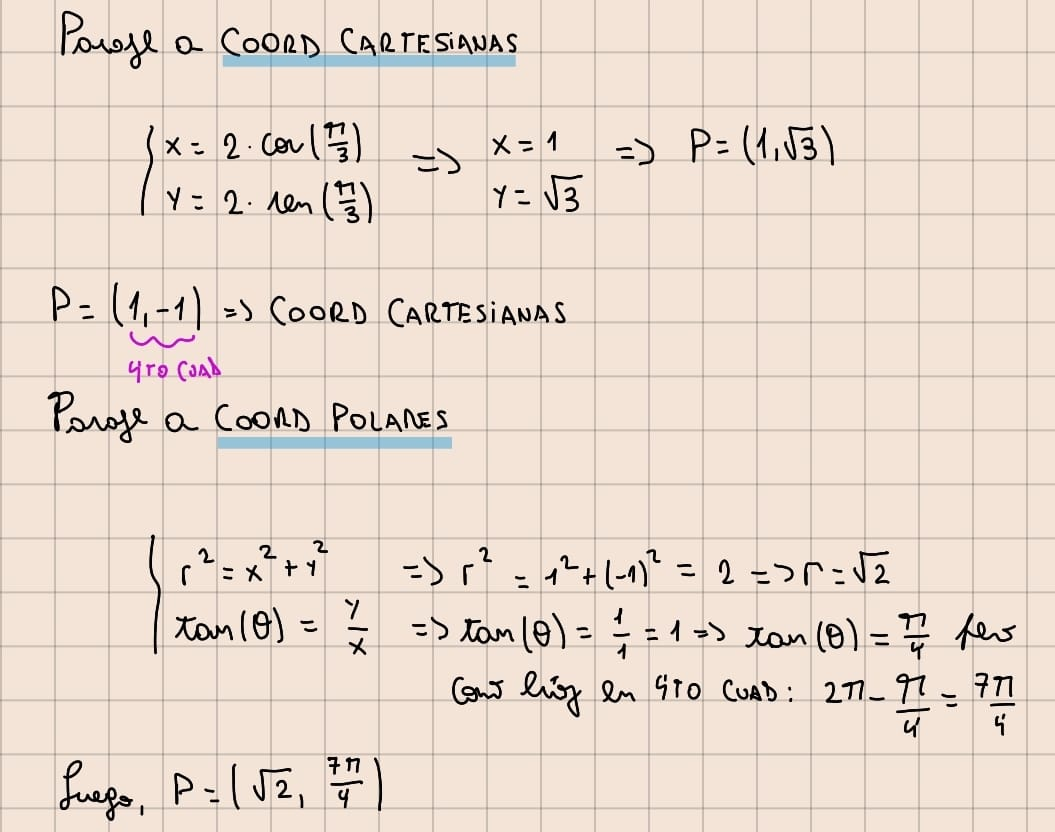
\includegraphics[width=\linewidth]{assets/pasaje_coord_polares_cartesianas.jpg}
\end{minipage}\]
\subsection*{Elipses}
\label{subsec:elipses_ejercicios}
\[\begin{minipage}[b]{0.7\textwidth}
    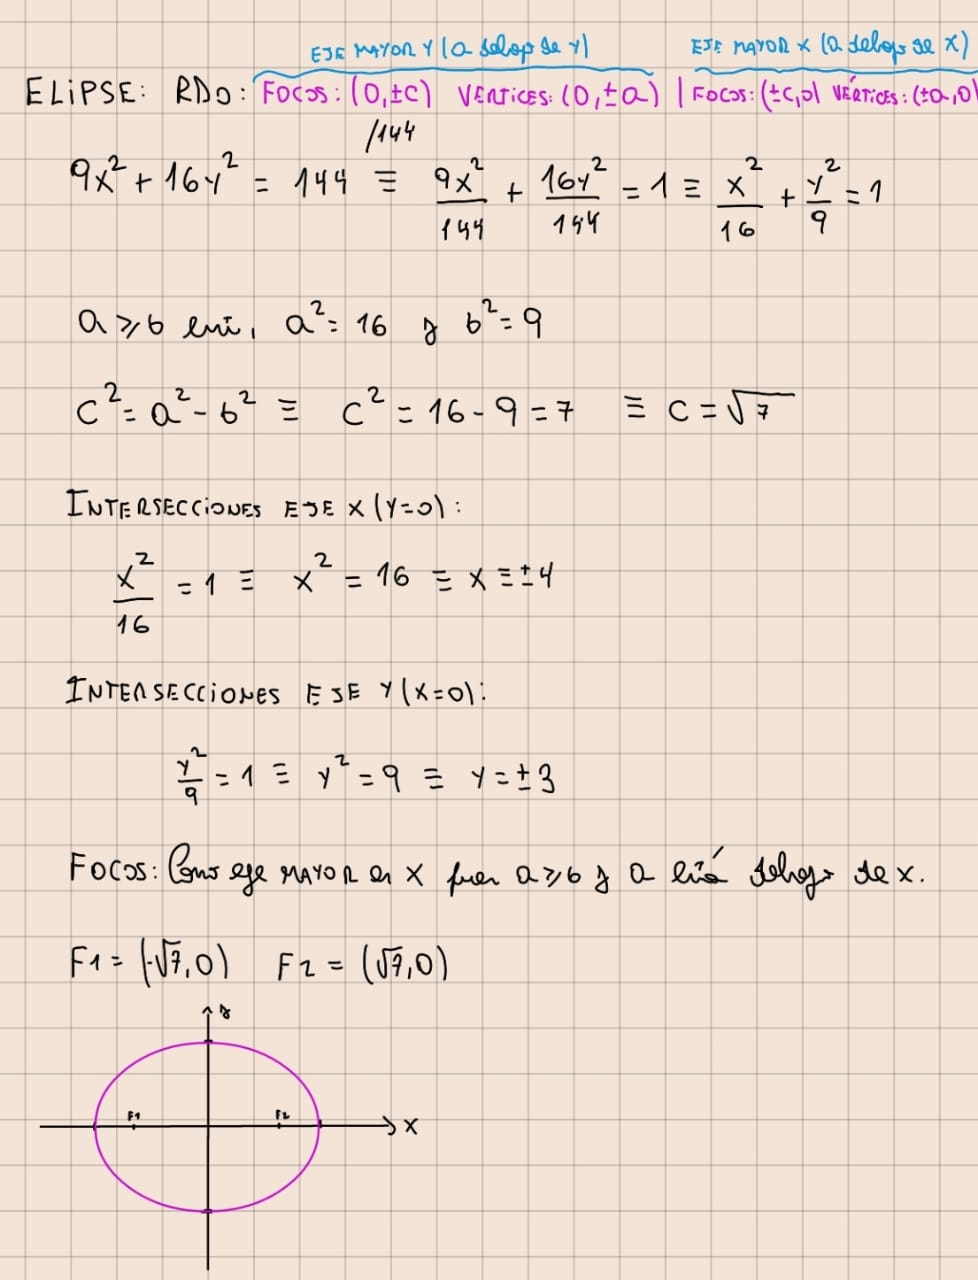
\includegraphics[width=\linewidth]{assets/elipse_1.jpg}
\end{minipage}\]
\[\begin{minipage}[b]{0.7\textwidth}
    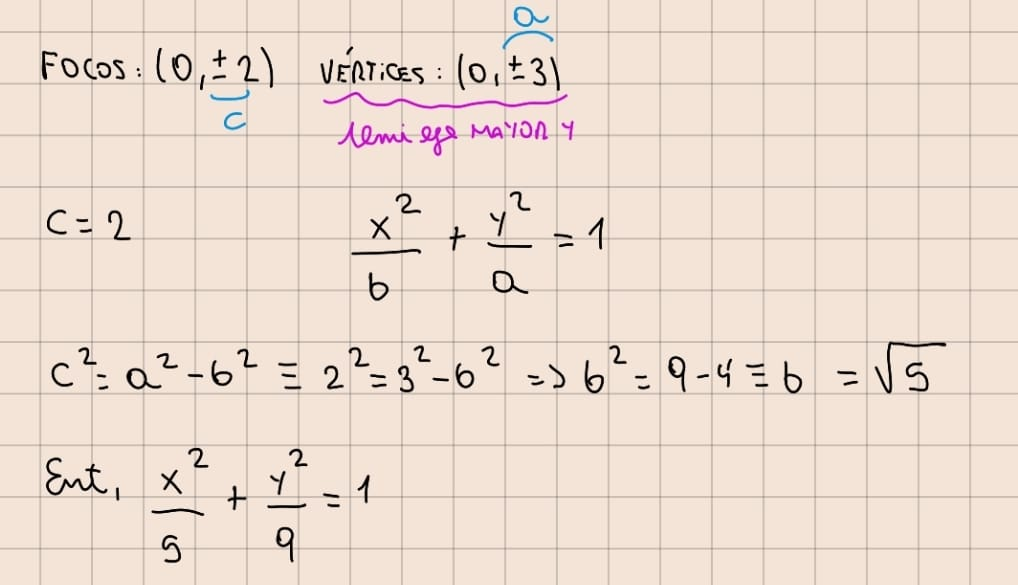
\includegraphics[width=\linewidth]{assets/elipse_2.jpg}
\end{minipage}\]
\subsection*{Hipérbolas}
\label{subsec:hiperbolas_ejercicios}
\[\begin{minipage}[b]{0.7\textwidth}
    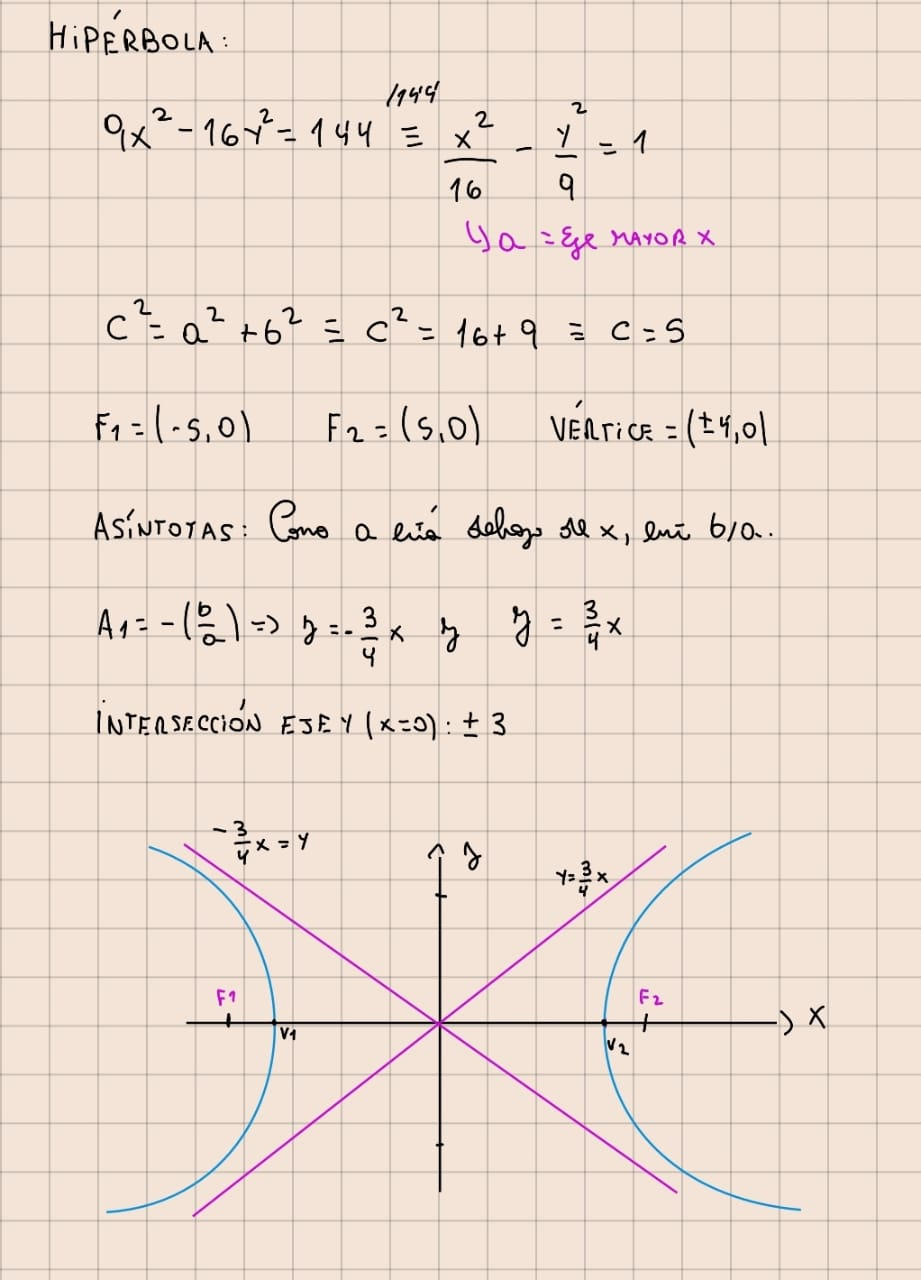
\includegraphics[width=\linewidth]{assets/hiperbola_1.jpg}
\end{minipage}\]
Con cónicas desplazadas y completar cuadrados
\[\begin{minipage}[b]{0.7\textwidth}
    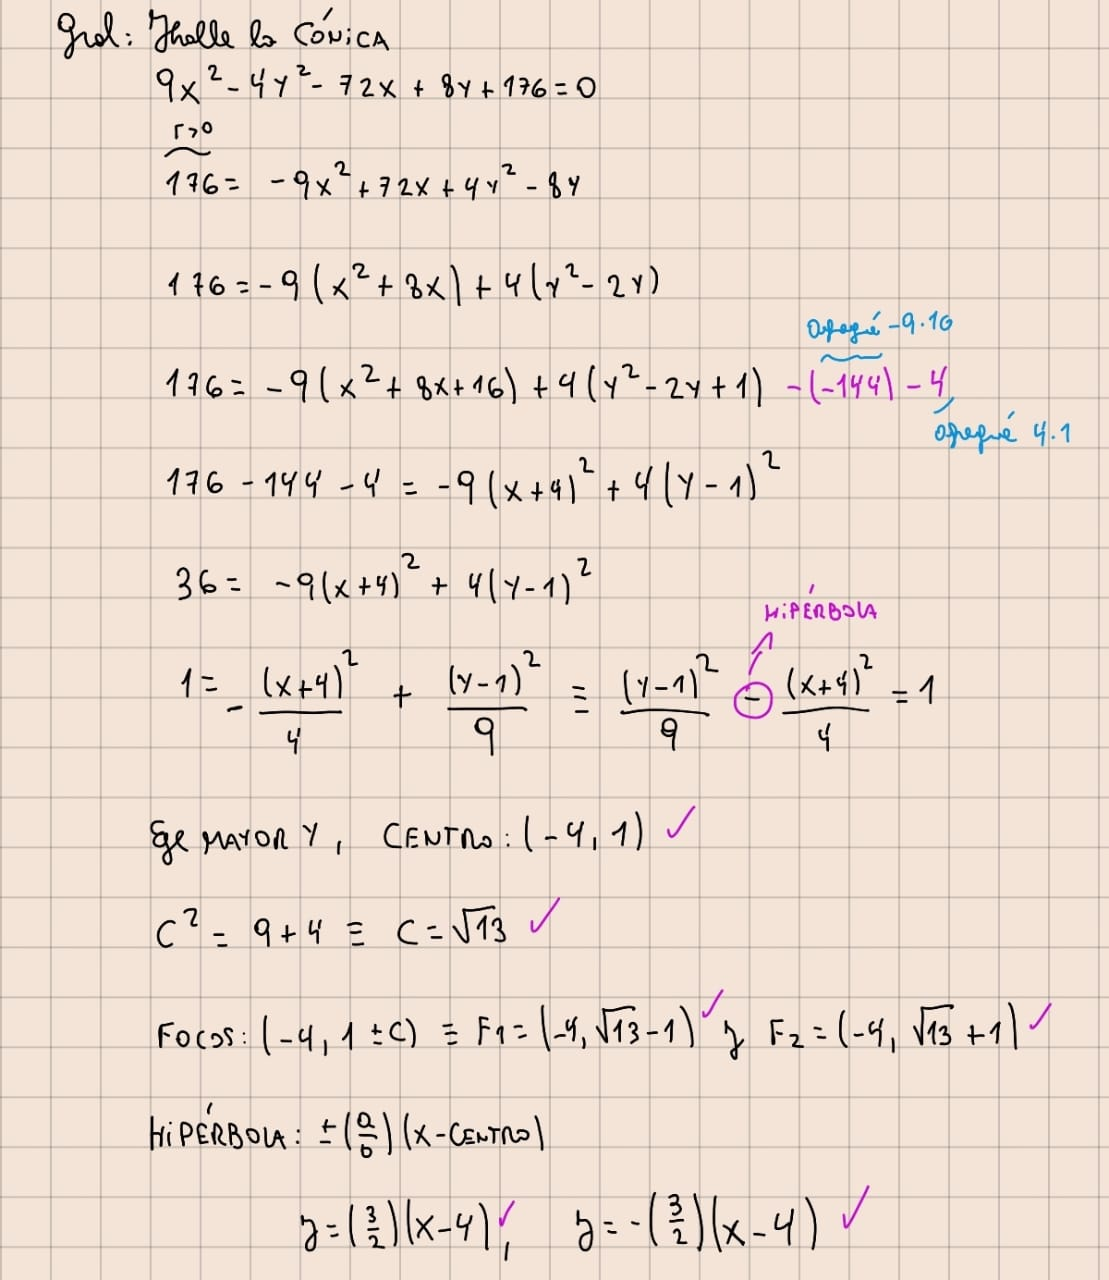
\includegraphics[width=\linewidth]{assets/hiperbola_2.jpg}
\end{minipage}\]

\end{document} 
